\chapter{A Higher Order Theory of Locality}
\label{chap:model}

An influential theory developed over the past four decades is the
working-set theory (WSLT)~\cite{Denning:TSE80}. In this chapter, we
develop a similar theory for cache locality (CLT), a higher order
theory of locality which connects five different locality metrics,
footprint, inter-miss time, volume fill time, miss ratio, and reuse
distance. The theory includes a series of conversion methods and their
correctness condition. We refer to the new theory as HOTL(a {\bf
  H}igher {\bf O}lder {\bf T}heory of {\bf L}ocality) theory and refer
to these methods collectively as the HOTL conversion for the five
metrics.

Footprint plays an important role in HOTL theory. The fact that
HOTL theory endows each of the five cache locality metrics the
collective strength of all its Filmer peers makes footprint's strength,
such as measuring efficiency and composibility, available to all other
metrics. HOTL theory can be used in many locality related fields, such
as locality measurement, prediction, and optimizations, in both
standalone and multi-tasks environments. 

\section{Introduction}
The memory system of a computer is organized as a hierarchy.  Locality
metrics are used in software and hardware to manage and optimize the
use of the memory hierarchy.  For locality analysis, the basic unit of
information is a data access, and the basic relation is a data reuse.
The theory of locality is concerned with the fundamental properties of
data accesses and reuses, just as the graph theory is with nodes and
their links.

Cache locality metrics are many and varied.  To quantify performance,
we use the miss rate.  To manage sharing, we use the footprint.  To
analyze and optimize a program, we use the reuse distance.  Some
metrics are hardware dependent, useful for evaluating a specific
machine and managing it at run time.  Others are hardware independent,
useful for optimizing a program for all cache sizes.  The two types of
metrics are converging in multicore caching, where the total cache
size is fixed but the available portion for each program varies. 

In this chapter we consider five locality metrics, with a short description
here and the precise definitions in the next section.

\begin{itemize}
\item \emph{Footprint}: the expected amount of data a program accesses
  in a given length window.
\item \emph{Inter-miss time}: the average time between two cache
  misses in a given size cache.
\item \emph{Volume fill time}: the average time for the program to
  access a given volume of data.
\item \emph{Miss ratio}: the fraction of references that cause cache
  misses.
\item \emph{Reuse distance}: for each data access, the amount of data
  accessed between this and the previous access to the same datum.
\end{itemize}

\noindent To denote them collectively, we insert `et' between the last
two,  take the initial letters (except for the fill time from which we
take one 'l'), and produce the acronym ``Filmer''. 

We present a theory showing that the five Filmer
metrics can be mutually derived from each other.  The conversion
involves taking the difference in one direction and the sum in the
reverse direction.  The theoretical relation is analogous to
differentiation and  integration.  Hence we call it a \emph{higher
  order theory} of locality (HOTL).

Similar conversions have been part of the working set theory, making
it the first HOTL theory (Section~\ref{sec:Denning}).  The working set
theory was developed to analyze locality in the main memory.  The new
theory we develop is for cache memory.  It endows each of the five cache locality
metrics the collective strength of all its Filmer peers:

\begin{itemize}
\item \emph{Efficiency}.  If we can measure one
  Filmer metric on-line, we can calculate all the others at the same
  time.
\item \emph{Composability}.  The miss rate does not compose in that
  when a group of programs are run together, the number of misses is
  not the sum of the misses of each member running alone.  If another
  Filmer metric is composable, then we can compose the miss rate
  indirectly.
\item \emph{Hardware sensitivity}.  If we can measure the effect of
  cache associativity and other hardware parameters on the miss rate,
  we can compute their impact on the other metrics.
\end{itemize}

The conversion methods we describe are not always accurate.  The
correctness depends on whether the footprint statistics in reuse
windows is similar to the footprint in general windows, in other
words, whether the reuse windows are representative of general
windows.  We call the condition the \emph{reuse-window hypothesis}.
The Filmer metrics capture different aspects of an execution: the
reuse distance is per access, the footprint is per window, while the
miss-ratio has the characteristics of both. Their conversion creates
conflicts, and the reuse-window hypothesis is the condition
for reconciliation.

We apply the HOTL theory to convert footprint to reuse distance and predict
the miss ratio. The purpose of the miss-ratio prediction is twofold:
to validate the theory and to show a practical value. The main results
are: 

\begin{itemize}
\item \emph{Real-time locality measurement.}  The HOTL-enabled
  technique predicts the miss ratio for thousands of cache sizes with
  a negligible overhead.  When tested on SPEC 2006 and
  PARSEC parallel benchmarks, the prediction matches the actual miss
  ratio measured using the hardware counters.  Without sampling, the
  analysis is 39\% faster than simulating a single cache size.  With
  sampling, the end-to-end slowdown is less than 0.5\% on average with
  only three programs over 1\%.

\item \emph{Cache interference prediction.} The HOTL-enabled technique
  predicts the effect of cache sharing without parallel testing.  We
  will focus on cache sharing models and present the results of
  applying HOTL theory to cache interference prediction in Chapter~\ref{chap:corun}.
\end{itemize}

Knowing the miss rate does not mean knowing the memory performance.
The actual effect of a cache miss depends significantly on data
prefetching, memory-bus arbitration, and other factors either in the
CPU above the cache hierarchy or the main memory below.  In this
chapter, we limit our scope to the models of data and cache usage and to
methods that measure and reduce the number of cache misses.

\section{Locality Metrics}
\label{sec:metrics}

The working set theory defines the locality metrics to measure the
intrinsic demand of a process~\cite{Denning:CACM68}.   The actual
performance is the hardware response to the program demand.  By
defining locality metrics independent of their specific uses, the
approach combines clarity and concision on the one hand and usefulness
and flexibility on the other. We follow the same approach and say that
a locality metric is \emph{program intrinsic} if it uses only the
information from the data access trace of a program.  Throughout this
chapter, we use $n$ to denote the length of the trace and $m$ the
total amount of data accessed in the trace. 

A footprint is defined on a time window, and the miss ratio for a
cache size.  Since we do not know a priori in which window or
cache the metrics may be used, we define the footprint and miss ratio
metrics to include all windows and all cache sizes --- they are
functions over a parameter range.

The five metrics we consider are program intrinsic functions defined
on a sequential data access trace.  The time is logical and counted by
the number of data accesses from the start of the execution.  The
cache is fully associative and uses the LRU replacement, with a fixed
cache-block size.  We will consider the physical time and set
associative cache when we apply the basic theory in
Chapter~\ref{chap:corun}.  We use the term miss ratio if the time is
logical and miss rate if it is physical. 

\subsection{Average Footprint}

In this section we briefly review the concepts and algorithms we
introduced in Chapter~\ref{chap:fp}, a footprint is the amount of data
accessed in a time window.  A performance tool often measures it for
some execution window, i.e. taking a snapshot.  A complete measure
should consider \emph{all} execution windows.  For each length $t$,
the average footprint $fp(t)$ is the average footprint size in all
windows of length $t$. 

Let $W$ be the set of all length-$t$ windows in a length-$n$ trace.
Each window $w$ has a footprint $fp_w$. The average footprint $fp(t)$
is the total footprint in these windows divided by $n-t+1$, the number
of the length-$t$ windows. 

$$fp(t) = \frac{\sum_{all\ w\ of\ length\ t} fp_w}{n-t+1}$$

For example, the trace ``abbb'' has 3 windows of length 2: ``ab'',
``bb'', and ``bb''.  The size of the 3 footprints is 2, 1, and 1, so
$fp(2) = (2+1+1)/3 = 4/3$.  

The footprint is composable in that the combined footprint of two
programs is the sum of their individual footprints (assuming no data
sharing).  We will use this property when developing efficient models
of cache sharing in Chapter~\ref{chap:corun}. Another useful property,
which we have already explored in Section~\ref{sec:sampling}, is that
the footprint is amenable to sampling.

\subsection{Volume Fill Time}
\label{subsec:lf}

Intuitively, we may consider the cache as a reservoir and the data
access of a program a stream feeding into the reservoir with new
content.  Having a fixed capacity, the reservoir discharges (evicts)
previous volumes as it receives the new flows.  The key concept in
this analogy is the volume fill time, the time taken for a stream to
fill the reservoir.

The volume fill time is the time a program takes to access a given
amount of data, or symbolically, $vt(v)$ for volume $v$.  The metric
is program intrinsic.  To model hardware, we simplify and assume that
the cache is fully associative LRU.  Under the assumption, the volume
fill time $vt(c)$ is the time for a program to fill the cache of size
$c$.  Whether the cache is empty or not, after $vt(c)$, the cache
is populated with the data (and only the data) accessed in the last
$vt(c)$ time. In the cold-start cache, all data will be brought in by
cache misses. In the warm cache, the fraction of the data already in
the cache will stay, and the rest will be brought in by cache
misses. We call the volume fill time interchangeably as the
\emph{cache fill time}. 

The fill time can be defined in two different ways. First, we define
it as the inverse of the footprint function:

\begin{align*}
vt(c) = 
\begin{cases}
fp^{\ -1} (c) & \text{if } 0 \le c \le m \\
\infty & \text{if } c > m
\end{cases}
\end{align*}

\noindent where $m$ is the total amount of program data. Within the
range $0 \le c \le m$, the invariant $fp(vt(c)) = fp(fp^{\ -1}(c))= c$
symbolizes the conversion that when the footprint is the cache size,
the footprint window is the fill time. The conversion is shown
visually in Figure~\ref{fig:fp2vt}.  From the average footprint curve,
we find the cache size $c$ on the y-axis and draw a level line to the
right.  At the point the line meets the curve, the $x$-axis value is
the fill time $vt(c)$.

A careful reader may question the uniqueness of the fill time.  For
example for the trace ``xx...x'', it is unclear what should be the fill
time $vt(1)$.  When defined as the inverse function $fp^{-1}$, the same
problem happens if there are $x_1,x_2$ such that $fp(x_1) = fp(x_2)$.
However, this problem does not occur using the footprint-based
definition.  We will prove later in Section~\ref{sec:thm} that the
average footprint is a concave function.  As a result, it is strictly
increasing, and as its inverse, $vt$ is a proper function and strictly
increasing as well.  We call the footprint-based
definition the \emph{Filmer fill time}.

\begin{figure}[t!]
\centering
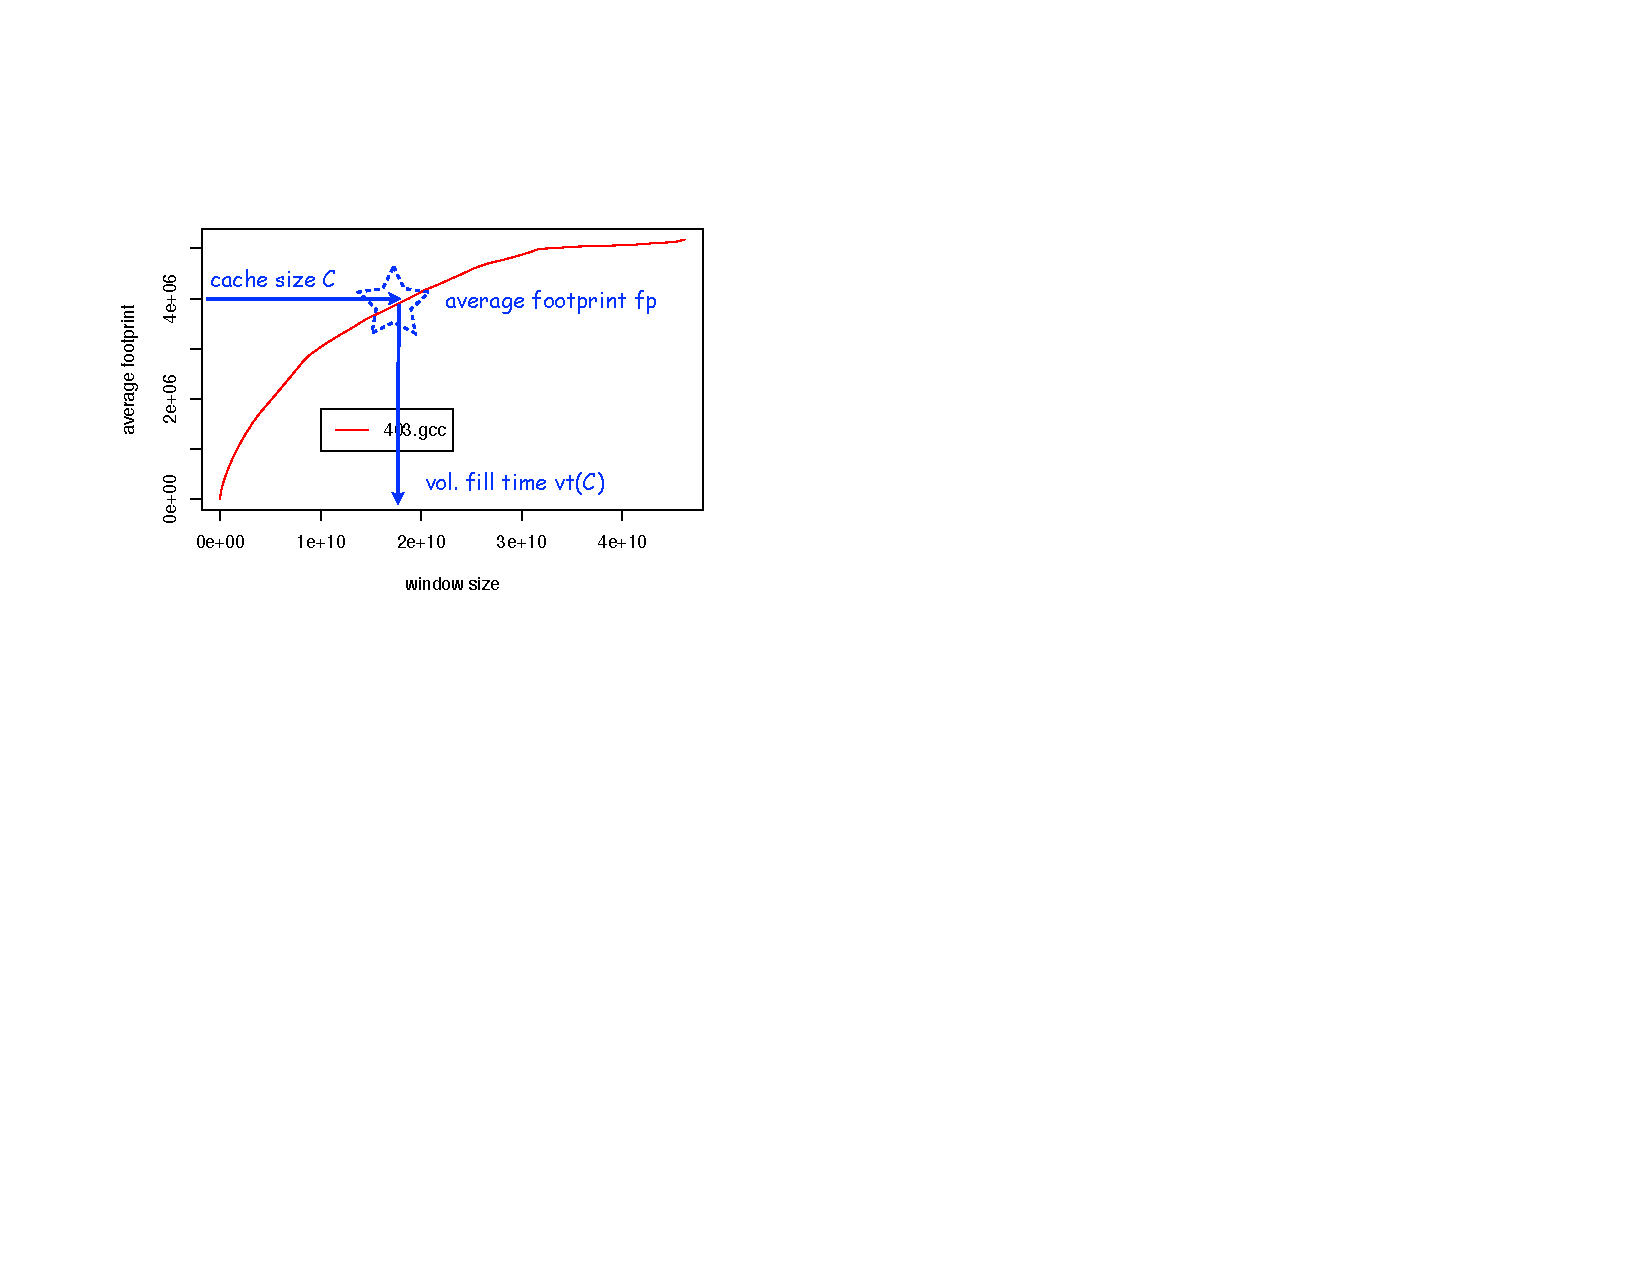
\includegraphics[width=0.7\textwidth]{figures/model/fp2vt.pdf}
\caption{Defining the volume fill time using the footprint.}
\label{fig:fp2vt}
\end{figure}

Alternatively, we can define the fill time in a different way.  For
the volume $v$, we find all windows in which the program
accesses $v$ amount of data.  The average window length is then the
fill time.We refer to the second definition the \emph{direct fill
  time}, since it is defined directly, not through function inversion.

Consider another example trace ``abbc''. The Filmer fill time is
$vt_{Filmer}(1) = 1$, since all single-element windows access one
datum.  The direct fill time takes the 5 windows with the unit-size
data access: ``a'', ``b'',``b'', ``bb'', and ``c'' and computes the
average $vt_{direct}(1) = (1+1+1+2+1)/5 = 6/5$. The Filmer definition
uses the windows of the same length.  The direct definition uses the
windows of possibly different lengths.

The cache fill time is related to the residence time in the working
set theory~\cite{Denning:TSE80}.  Once a program accesses in a data
block but stops using it afterwards, its residence time in cache is
the time it stays in cache before being evicted.

For a trace of $n$ accesses to $m$ data, the direct fill time can be
measured by an algorithm that counts all $O(n^2)$ windows but reduces
the quadratic cost of counting in three ways.  The solution is similar
in design to all-window footprint measurement as introduced in
Section~\ref{sec:all-fp}. However, the direct definition has serious
flaws, the predicted miss ratio is not monotone.  Worse, the miss
ratio may be negative.  Consider an example trace with 100 a's
followed by 11 b's, 1 c, 20 d's, 15 e's, 1 f and 320 g's.  The average
time to fill a 4-element cache, $vt(4)$, is 161.5, is longer than the
average time to fill a 5-element cache, $vt(5)$, which is 149.5.
Since the direct fill time decreases when the cache size $v$
increases, the predicted miss ratio is negative! 

The preceding example was constructed based on an analysis of real
traces.  During experimentation, we found that the miss ratios of some
cache sizes were negative.  While most of the 3000 or so sizes
had positive predictions, the negatives were fairly frequent and happened in
most test programs.  It seemed contradictory that it could take a
program longer to fill a smaller cache.  The reason is
subtle.  To compute the direct fill time, we find windows with the same
footprint and take the average length.  As we increase the footprint
by 1, the length of these windows will increase but the number of such
windows may increase more, leading to a lower average, as happened in
the preceding example.

In contrast, the Filmer fill time is a positive, concave function
(Corollary~\ref{concavity}).  Its miss-ratio prediction is monotone and
can be measured in near real time (Section~\ref{sec:samp-result}).
Unless explicitly specified in the rest of the chapter, by
fill time we mean the Filmer fill time.

\subsection{Inter-miss Time and Miss Ratio}
\label{subsec:mr}

We derive the inter-miss time for fully associative LRU cache of size
$c$. Starting at a random spot in an execution, run for time $vt(c)$,
the program accesses $c$ amount of data and populates the cache of
size $c$.  It continues to run and use the data in the cache until the
time $vt(c+1)$, when a new data block is accessed, triggering a
capacity or a compulsory miss~\cite{Hill:Dissertation}.  The time
interval, $vt(c+1) - vt(c)$, is the miss-free period when the program
uses only the data in cache.  We use this interval as the average
inter-miss time $im(c)$\footnote{In the working-set theory, the
  corresponding metric is the time between page faults and known as
  the lifetime.}.  The reciprocal of $im(c)$ is the miss ratio
$mr(c)$.

\begin{align*}
im(c) = 
\begin{cases}
vt(c+1)-vt(c) & \text{if } 0 \le c < m \\
\frac{n}{m} & \text{if } c \ge m
\end{cases}
\end{align*}

Since the fill time is the inverse function of the footprint, we can
compute the miss ratio from the footprint directly. The direct
conversion is simpler and more efficient. In practice, we measure the
footprint not for all window sizes but only those in a logarithmic
series.  Let $x$ and $x+\Delta x$ be two consecutive window sizes we
measure, we then compute the miss ratio for cache size $c = fp(x)$:

\begin{align*}
mr(c) = mr(fp(x)) = \frac{fp(x+\Delta x) - fp(x)}{\Delta x}
\end{align*}

\noindent 

Being a simpler and more general formula, we will use it in the theoretical
analysis and empirical evaluation.  To cover all cache sizes in practice, we use it as
the miss ratio for all cache sizes $c \in [fp(x), fp(x+\Delta x))$.

The fill time ($vt$) conversion and the footprint ($fp$) conversion
are equivalent.  Figure~\ref{fig:fp2mr} shows the two visually.  For
the same two data points on the footprint curve, let $\Delta x = x_2 -
x_1$ be the difference in the window length and $\Delta y = y_2 - y_1$
be the difference in the amount of data access.  The fill time
conversion computes the inter-miss time $im(y_1) = \frac{vt(y_2) -
  vt(y_1)}{y_2 - y_1} = \frac{\Delta x}{\Delta y}$, and the footprint
conversion computes the miss ratio $mr(fp(x_1)) = mr(y_1) =
\frac{fp(x_2) - fp(x_1)}{x_2 - x_1} = \frac{\Delta y}{\Delta x}$.

\begin{figure}[t!]
\centering
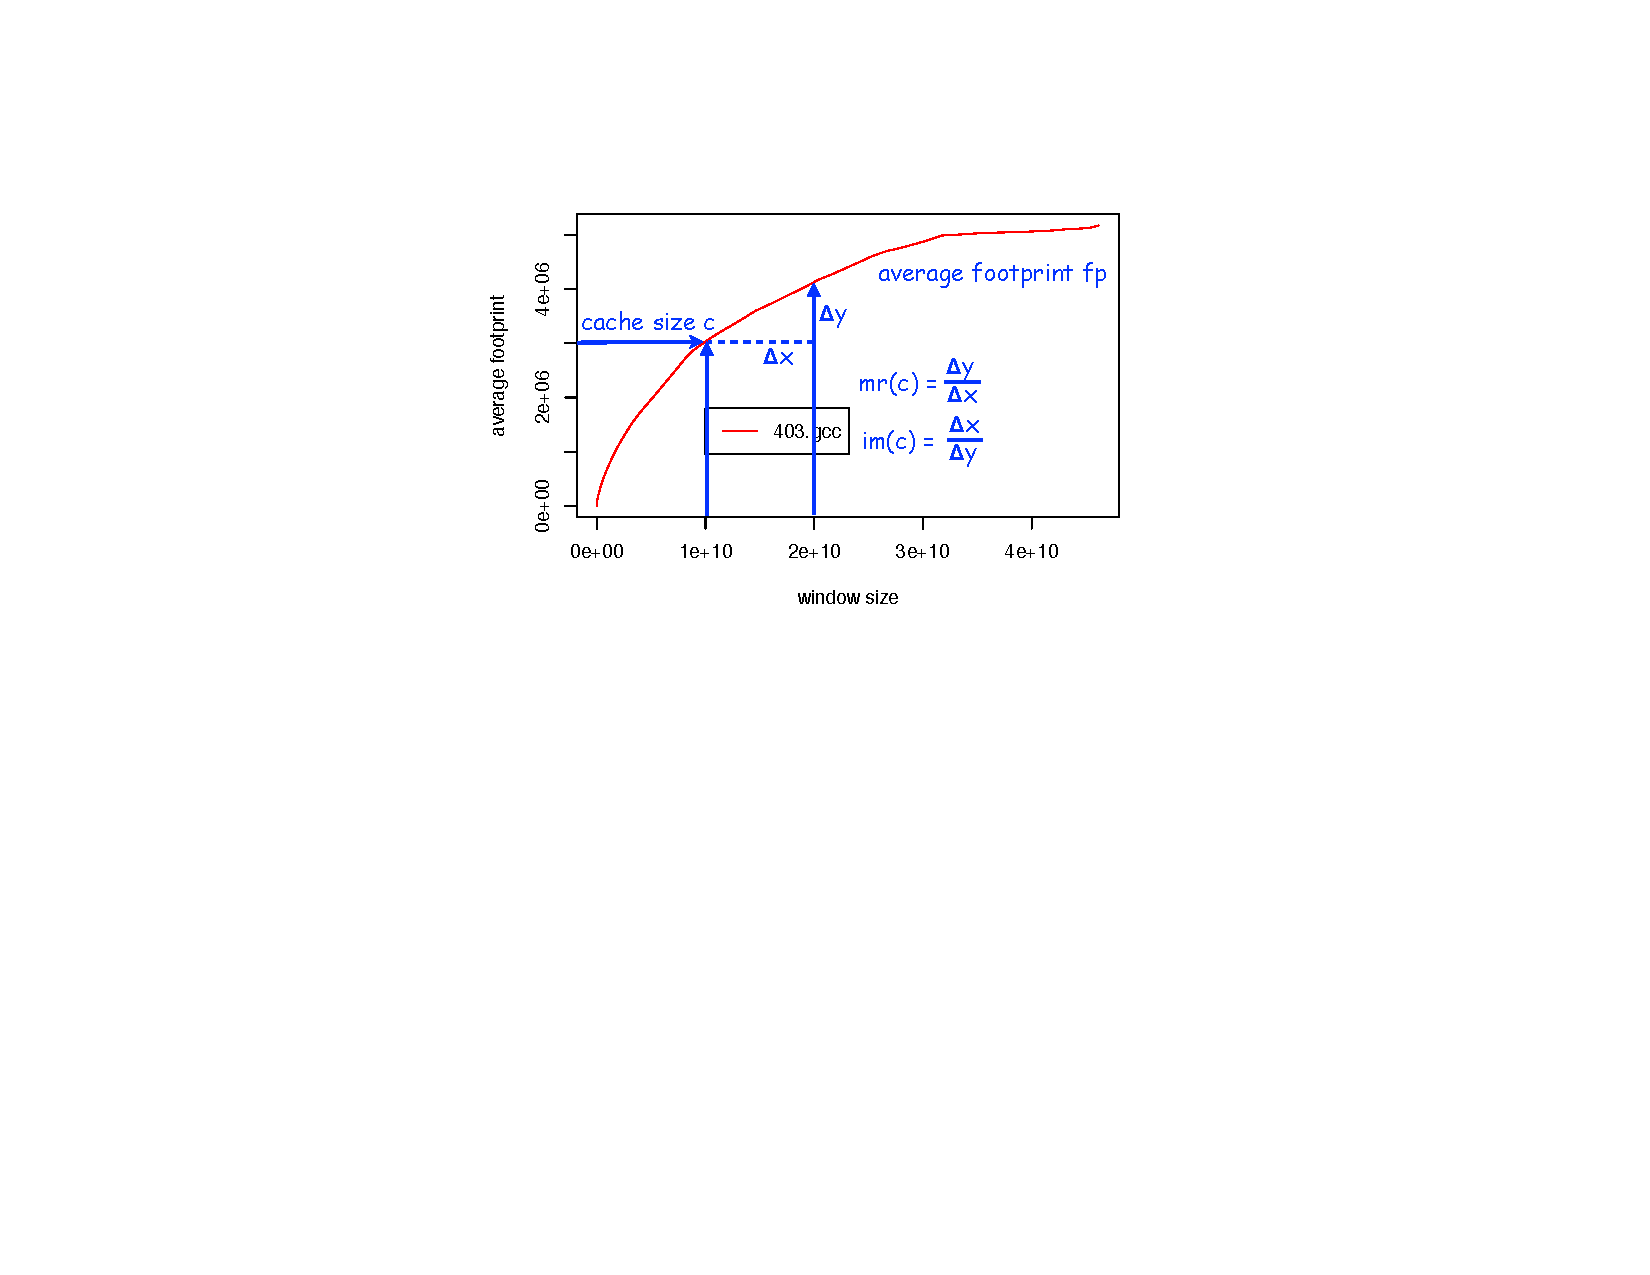
\includegraphics[width=0.7\textwidth]{figures/model/fp2mr.pdf}
\caption{Equivalent conversions of the footprint to the
  miss ratio and the fill time to the inter-miss time.}
\label{fig:fp2mr}
\end{figure}

For associative cache, Smith showed that cache conflicts can be
estimated based on the reuse distance~\cite{Smith:ICSE76}.  Hill and Smith
evaluated how closely such estimate matched with the result of cache
simulation~\cite{HillS:TOC89}.  We next derive the reuse distance.
Once derived, we can use it and the Smith formula to estimate the
effect of cache conflicts and refine the miss ratio prediction.

\subsection{Reuse Distance}

For each memory access, the {\em reuse distance}, or \emph{LRU stack
  distance}, is the number of distinct data used between this and the
previous access to the same datum~\cite{Mattson+:IBM70}.  The reuse
distance includes the datum itself, so it is at least 1. The
probability function $P(rd=c)$ gives the fraction of data accesses
that have the reuse distance $c$.  The capacity miss ratio, $mr(c)$,
is the total fraction of reuse distances greater than the cache size
$c$, i.e. $mr(c)=P(rd > c)$. Consequently, 

\begin{align*}
P(rd=c) = mr(c-1) - mr(c)
\end{align*}

The reuse distance has extensive uses in program analysis and locality
optimization.  Any transformation that shortens a long reuse distance
reduces the chance of a cache miss. At the program level, reuse
distance analysis extends dependence analysis, which identifies reuses
of program data~\cite{AllenK:Book01}, to count the volume of the
intervening data~\cite{CascavalP:ICS03,BeylsD:JSA05,ChauhanS:ICS10}.
At the trace level, the analysis can correlate the change in locality
in different runs to derive program-level patterns and complement
static analysis~\cite{Zhong+:TOPLAS09,MarinM:SIGMETRICS04,Fang+:CC06}.

\bigskip
To review the conversion formulas, let's consider the example trace
``xyzxyz...''.  Assuming it infinitely repeating, we have $m=3$ and
$n=\infty$.  Table~\ref{tbl:filmer-eg} shows the discrete values of
the Filmer metrics computed according to the HOTL conversion.

\begin{table}
\centering
%\renewcommand{\arraystretch}{1.4}
\begin{tabular}{|cc|ccccc|}
\hline
$t$ & $fp(t)$ & $c$ & $vt(c)$ & $im(c)$ & $mr(c)$ & P(rd=c) \\ \hline
1 & 1 & 1 & 1 & 1 & 1 & 0\\
2 & 2 & 2 & 2 & 1 & 1 & 0  \\
3 & 3 & 3 & 3 & $\infty$ & 0 & 1 \\
4 & 3 & 4 & $\infty$ & $\infty$ & 0 & 0\\ \hline 
\end{tabular}
\caption{Discrete values of the Filmer metrics computed according to
  the HOTL conversion}
\label{tbl:filmer-eg}
\end{table}

\section{The Higher Order Relations}
\label{sec:relations}

In algebra, the term order may refer to the degree of a polynomial.
Through differentiation, a higher order function can derive a lower
order function.  If we use the concept liberally on locality functions
(over the discrete integer domain), we see a higher order locality
theory, as shown in a metrics hierarchy in Figure~\ref{fig:theory}.

\begin{figure}[h!]
\centering
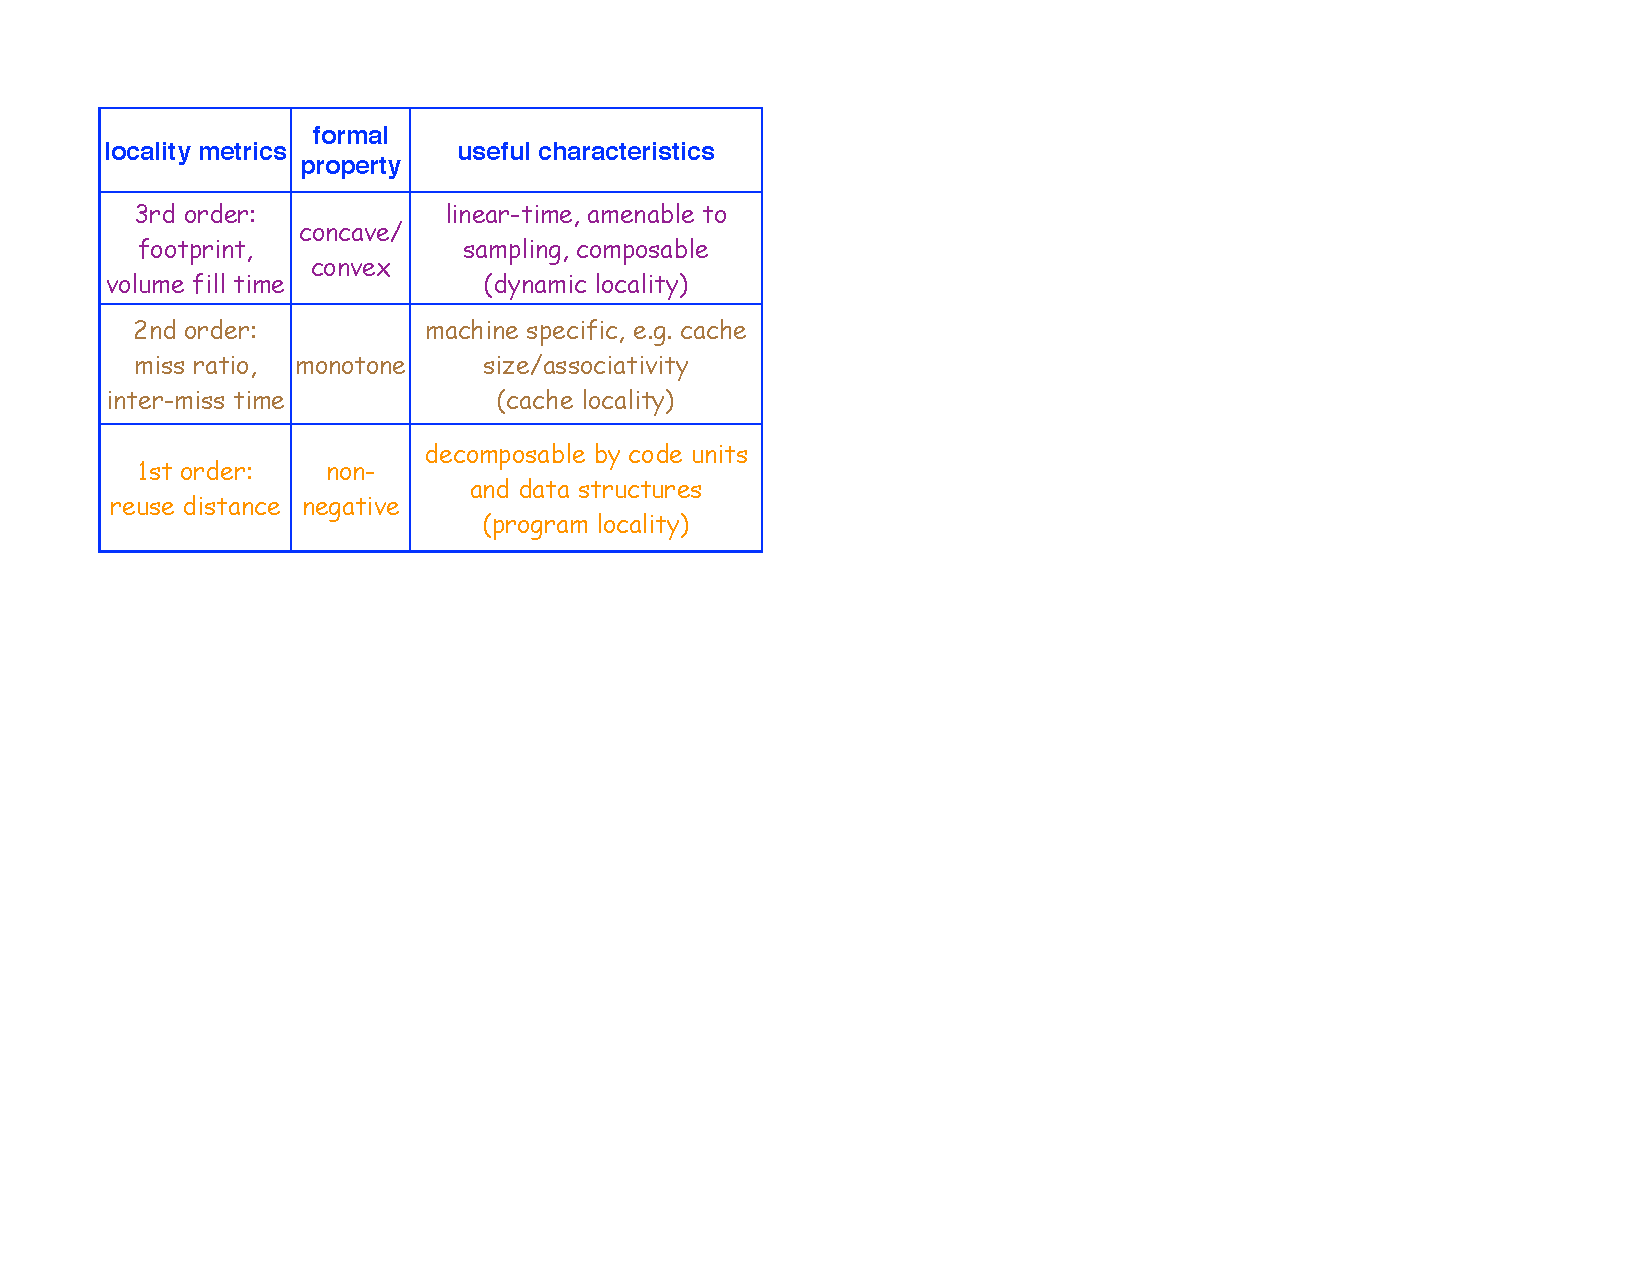
\includegraphics[width=0.7\textwidth]{figures/model/theory}
\caption{The hierarchy of cache locality metrics.  The five locality metrics are
  mutually derivable by either taking the difference of the metrics
  when moving down the hierarchy or taking the sum of the metrics 
  when moving up.}
\label{fig:theory}
\end{figure}

In the preceding sections, we have shown the series of conversions
from the third order metric, the footprint, to the first order metric,
the reuse distance.  To compute a lower order metric, the HOTL
conversion takes the difference of the function of a higher order
metric.  The inter-miss time is the difference of the fill times, and
the reuse distance is the difference of the miss ratios. 

The conversion formulas are all reversible.  We can calculate a higher
order metric by integrating the function of a lower order metric. For
example, the miss ratio is the sum of the reuse distances greater than
the cache size.  The fill time is the sum of the inter-miss times up
to the cache size.

The mathematical property is different depending on the order of the
locality metric, as shown in the second column in
Figure~\ref{fig:theory}.  Going bottom up, the reuse distance is a
distribution, so the range is non-negative.  For just compulsory and
capacity misses, the miss ratio is monotone and non-increasing,
i.e. the stack property~\cite{Mattson+:IBM70}.  The footprint has been
shown to be monotone(Section~\ref{subsec:aver-fp-mono}).  Later we will prove
a stronger property. 

Although the phrase “higher order” was not used, the working set
theory was about the higher order relations between the working set
size, the miss rate, and the reuse-time interval.  In
Section~\ref{sec:Denning}, we will compare the two higher order
theories. 

\section{The Correctness Condition}
\label{sec:thm}

The conversion from the footprint to the miss ratio is not always
correct.  To understand correctness, consider the reuse distance and
the footprint both as window statistics.  The reuse distance is the
footprint of a reuse window.  A reuse window starts and finishes with
two accesses to the same datum with no intervening reuses. For a
program with $n$ accesses  to $m$ data, there are $n-m$ finite-length
reuse windows. They are a subset of all windows.  The number of all
windows is $n$ choose 2 or $\frac{n(n+1)}{2}$.  We define the average
footprint over all reuse windows as $rfp(l)$, the same way we define
$fp(l)$ over all windows.

In this section, we show the correctness condition: for the HOTL
conversions to be correct, the two functions, $fp(l)$ and $rfp(l)$,
must be equal. 

To show this result, we introduce a different formula for predicting
the miss ratio. To estimate whether an access is a miss for cache size
$c$, we take the reuse window length $l$, find the average footprint
$fp(l)$, and predict it a cache miss if and only if $fp(l) > c$.  We
call this method the \emph{reuse-time conversion}.  Let $P(rt=t)$ be
the density function of the reuse time, that is, the fraction of reuse
windows with the length $t$.  The miss ratio predicted by the
reuse-time conversion is as follows.  We label the result $mr_{rt}$ to
indicate that the prediction is based on the reuse time.  The first
access to a datum has the reuse time of $\infty$.

\begin{align*}
mr_{rt}( fp(l) ) = P(rt > l) = \sum_{t=l+1}^{\infty} P(rt = t)
\end{align*}

\noindent If we re-label $fp(l)$ as the working set size, the formula
is identical to that of Denning and Schwartz
(Section~\ref{sec:Denning}).  However, the use of $fp(l)$ is an
important difference.  The reuse-time conversion is a modified version
of Denning and Schwartz. We may call it an augmented Denning-Schwartz
conversion. 

Take the example trace ``xxyxxz''.  Two of the average footprints are
$fp(3) = 2$ and $fp(4) = \frac{7}{3}$.  The reuse times, i.e. the
length of the reuse windows, are $\infty, 2, \infty, 3, 2, \infty$.
The reuse-time conversion is $mr_{rt}( 2 ) = mr_{rt}(fp(3) ) =
\sum_{t=4}^{\infty} P(rt = t) = 50\%$. The Filmer conversion is based
on the footprint.  We call it $mr_{fp}$ and have $mr_{fp}( 2 ) = fp(4)
- fp(3) = 33\%$. In general for small traces, the reuse-time
conversion is more accurate, as is the case in this example.

\medskip

Next we prove that for large traces, the miss ratio prediction is the
same whether using the reuse time or using the footprint.  Then we
will show the correctness condition of the entire HOTL theory as a corollary.

From the view of the locality-metrics hierarchy, the reuse-time conversion is
bottom up from a first-order metric to a second-order metric.
The footprint conversion is top-down from a third-order metric to
the same second-order metric.  If they meet and produce the same result,
we have the equivalence relation across the entire hierarchy.

To prove the equivalence, we need the formula that computes the
average footprint from the reuse-time distribution introduced in
Section~\ref{sec:avg-fp}. 

\begin{lemma}[Average footprint formula]
\begin{eqnarray}
\label{eq1}
& fp(w)
&=m-\frac{1}{n-w+1}(\sum_{i=1}^{m}(f_i-w)I(f_i>w)+\sum_{i=1}^{m}(l_i-w)I(l_i>w)\nonumber
\\
& &r+\sum_{t=rw+1}^{n-1}(t - w)P(rt=t))
\end{eqnarray}
\label{eq:pact11}
\end{lemma}

\noindent The definitions of theses symbols can be found in
Section~\ref{sec:avg-fp}. If we assume $n \gg w$, the equation can be simplified to

$$fp(w) \approx m - \sum_{t=w+1}^{n-1}(t - w) P(rt=t) $$

\begin{theorem}[Footprint and reuse-time conversion equivalence] For
  long executions ($n \gg w$ ), the footprint conversion   and the
  reuse-time conversion produce equivalent miss-ratio predictions. 
\label{cteq}
\end{theorem}

\begin{proof}
  Let the cache size be $c$ and $l$ and $l+x$ be two consecutive window
  sizes such that $c \in [fp(l), fp(l+x))$. The miss ratio by the
    footprint conversion is $\frac{fp(l+x) - fp(l)}{x}$. Expand the
    numerator $fp(l+x)-fp(l)$ using the approximate equation from Lemma~\ref{eq:pact11}:
    
    \begin{align*}
      & fp(l+x) - fp(l) & 
      \approx & \sum_{t=l+1}^{n-1}(t - l) P(rt=t) - \sum_{t=l+x+1}^{n-1}(t - l -x) P(rt=t)\\
      & &= & \sum_{t=l+1}^{l+x}(t - l) P(rt=t) + x \sum_{t=l+x+1}^{n-1} P(rt=t) \\
      & &\approx & \sum_{t=l+1}^{l+x} x P(rt=t) + x \sum_{t=l+x+1}^{n-1} P(rt=t) \\
      & &= & x \sum_{t=l+1}^{n-1} P(rt=t) \\
      & &r\approx & x \sum_{t=l+1}^{\infty} P(rt=t) 
    \end{align*}

The miss ratio, $\frac{fp(l+x) - fp(l) }{x}$, is approximately
$\sum_{t=l+1}^{\infty} P(rt=t)$, which is the result of the reuse-time
conversion.  \qed 
\end{proof}

The two predictions being the same does not mean that they are
correct.  They may be both wrong.  Since the correct calculation can
be done using reuse distance, the correctness would follow if from the
reuse time, we can produce reuse distance.  In other words, the
correctness depends on whether the all-window footprint used by
the reuse time conversion is indeed the reuse distance.  We can phrase the
correctness condition as follows:

\begin{corollary}[Correctness] The footprint-based conversions are
  accurate if the footprints in all reuse windows have the same distribution
  as the footprints in all windows, for every reuse window length $l$.
\label{correctness}
\end{corollary}

\noindent When the two are equal, using the all-window footprint is
the same as using the reuse distance.  We posit as a hypothesis that
the condition holds in practice, so the HOTL conversion is accurate.
We call it the \emph{reuse-window hypothesis}.

\medskip

Consider the following two traces in Table~\ref{tbl:filmer-eg2}.  The
second trace has a smaller difference between the all-window footprint
$fp$ and the reuse-window footprint $rfp$.  The smaller difference
leads to more accurate miss ratio prediction by HOTL. The hypothesis
does not hold in either trace, so the prediction is not completely
accurate.  As to real applications, we will show an empirical
evaluation for the full suite of SPEC CPU2006 benchmark
programs~\cite{Henning:CPU2006} and a number of PARSEC parallel
programs~\cite{Bienia+:PACT08}. 

\begin{table}
\centering
\begin{tabular}{|c|c|c|c|c|c|}
\hline
    & & & \multicolumn{2}{|c|}{mr(1)} & error \\ \cline{4-5}
trace & $fp(2)$ & $rfp(2)$ & $pred$ & $real$ & $\lvert pred-real \rvert$ \\ \hline
wwwx & 4/3 & 1 & 1/3 & 2/4 & 17\%\\ \hline
wwwwx & 5/4 & 1 & 1/4 & 2/5 & 5\% \\ \hline
\end{tabular} 
\caption{A two-traces example showing the effect of reuse-window
  hypothesis on the accuracy of miss ratio prediction.}
\label{tbl:filmer-eg2}
\end{table}

\medskip

Finally, we show another consequence of Theorem~\ref{cteq}.

\begin{corollary}[Concavity] The average footprint $fp(x)$ is a
  concave function.
\label{concavity}
\end{corollary}

Since $\frac{fp(l+x) - fp(l) }{x} \approx \sum_{t=l+1}^{\infty}
P(rt=t)$, $fp(l)$ always increases but increases at a slower rate for
a larger $l$.  The function is obviously concave.  In the higher order
relation, the concavity guarantees that the miss ratio predicted by
HOTL is non-increasing with the cache size (as expected from the
inclusion property~\cite{Mattson+:IBM70}). 

\section{Comparison with Working Set Theory}
\label{sec:Denning}

The first higher-order locality theory is the working set theory,
pioneered in Peter Denning's thesis work~\cite{Denning:CACM68}.  His
1968 paper established the relation between the working set size, the
miss rate, and the inter-reference interval (iri).  The last one is
the same as reuse time.  The notion of reuse distance or the LRU
stack distance was not formalized until 1970~\cite{Mattson+:IBM70}. 
Figure~\ref{fig:hotl} shows the parallels between the working set locality theory (WSLT) 
and the new cache locality theory of this paper (CLT).

\begin{figure}[h!]
\centering
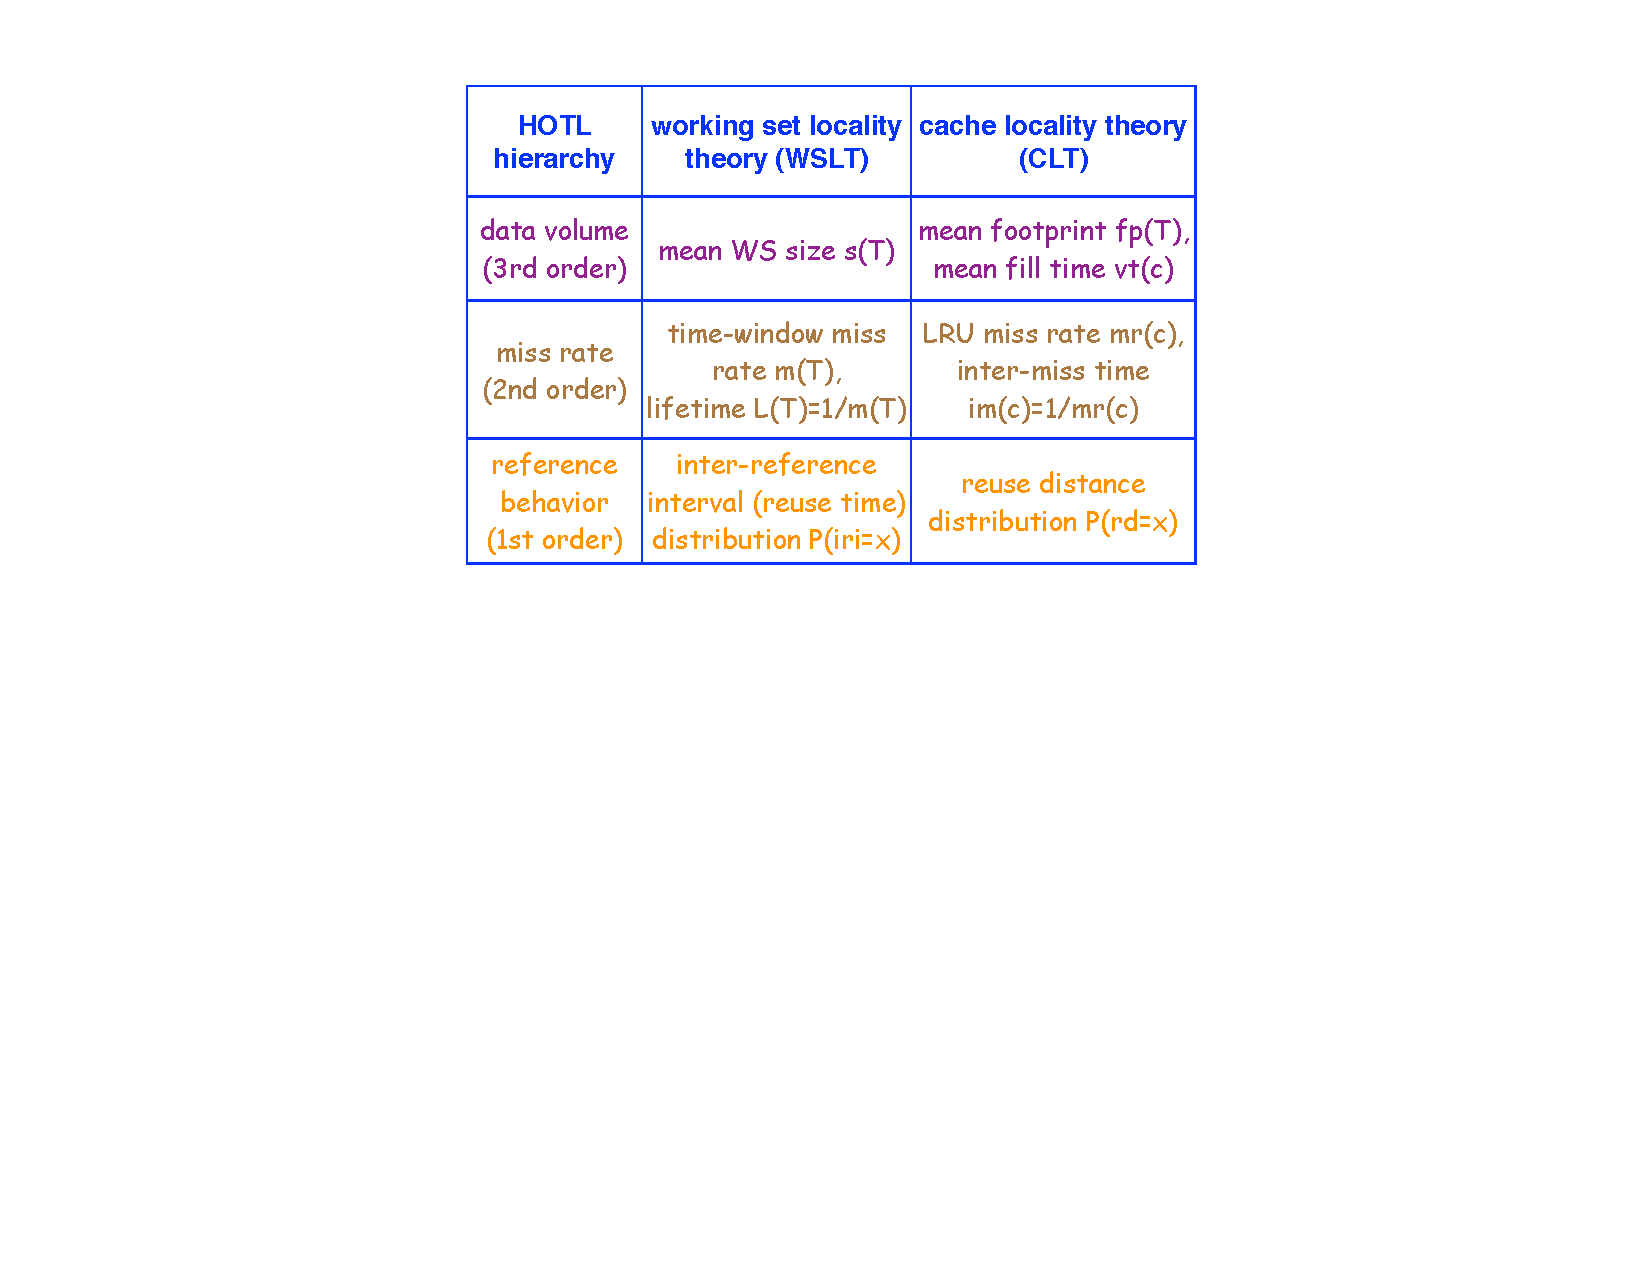
\includegraphics[width=0.7\textwidth]{figures/model/hotl}
\caption{Comparison between two higher order locality theories: the
  working set locality theory (WSLT) for dynamic partitioned primary
  memory and the cache locality theory (CLT) for cache memory.}
\label{fig:hotl}
\end{figure}

\noindent WSLT computes the metrics bottom-up.  The base metric,
$P(iri=x)$, is the histogram of the
inter-reference intervals (reuse time), measured in linear time in a
single pass of the address trace.  The time-window miss ratio $m(T)$ 
is the sum of reuse time.  The mean working set size $s(T)$ is
the sum of $m(T)$. 

\begin{align*}
m(T) = P(rt>T)\\
s(T+1) = s(T) + m(T)
\end{align*}

\noindent Taking together, the working set size $s(T)$ is the second
order sum of the reuse frequency.  

The $s(T)$ formula was first proved by Denning and Schwartz in
1972~\cite{DenningS:CACM72}.  The formulation assumes an infinitely
long execution with a ``stationary'' state (``the stochastic mechanism
... is stationary'').  The working set, $w(t,T)$, is the number of
distinct pages accessed between time $t-T+1$ and $t$.  The average
working set size, $s(T)$, is the limit value when taking the average
of $w(t,T)$ for all $t$.  The proof is based on the fact that only
recurrent pages with an infinite number of accesses contribute to the
mean working set size.

In 1978, Denning and Slutz defined the generalized working set (GWS)
as a time-space product~\cite{DenningS:CACM78}.  The product, denoted
here as $st(T)$, is defined for finite-length execution traces,
variable-size memory segments, all cache replacement policies that
observe the stack property.  Interestingly, they found the same
recursive relation.  The GWS formula is as follows, where the last
term is the extra correction to take into account the finite trace length.

$$st(T+1) = st(T) + Tm(T) - a(T)$$

\noindent Dividing both sides by $T$, we have the last term vanishing for large
$T$ and see the same recursive relation for GWS in finite-length traces as $s(T)$ in infinitely long
traces.

% emerges but not completely in view until now
In the present paper, the same recurrence emerges in Section~\ref{sec:thm} as an
outcome of Theorem~\ref{cteq}.  For the average footprint, we have
effectively

$$fp(T+1) = fp(T) + m(T) $$

If we view the following three as different definitions of the working set: the
limit value in 1972~\cite{DenningS:CACM72}, the time-space product in
1978~\cite{DenningS:CACM78}, and the average footprint in
2011~\cite{Xiang+:PACT11}, we see an identical equation which Denning
envisioned more than four decades ago (before the first proof in 1972).  We
state it as a law of locality and name it after its inventor:

% Denning's Law of Locality
\newenvironment{dlaw}[1][\sc \bf Denning's Law of
Locality]{\begin{trivlist} \item[\hskip \labelsep {\bfseries #1}]}{\end{trivlist}}


\begin{dlaw} \emph{The working set is the second-order sum of the reuse
  frequency, and conversely, the reuse frequency is the second-order
  difference of the working set.}
\end{dlaw}

As the relativity theory gives the relation between space and time,
Denning's law gives the relation between memory and computation: the
working set is the working memory, and the reuse frequency is a
summary of program actions (time transformed into frequency and a
spectrogram of time).  The law states that the relation is higher
order.

Our work augments Denning's law in two ways.  First, it is the final
step to conclusively prove Denning's Law --- that it holds for the
footprint working set in finite-length program executions.  The 1972
proof depends on the idealized condition in infinite-length
executions.  Subsequent research has shown that the working set theory
is accurate and effective in managing physical memory for real
applications~\cite{Denning:TSE80}. The new proof subsumes the
infinitely long case and makes Denning's law a logical conclusion for
all (long enough) executions.  It gives a theoretical explanation to
the long observed effectiveness of the working set theory in practice.

Second, we extend HOTL to include cache memory. For main memory, the
locality is parameterized in time: the working set of a program in a
time quantum.  For cache, the primary constraint is space: the miss
ratio for a given cache size.  Denning et al. named them the
``time-window miss ratio'' and the ``LRU miss ratio'' and noted that
the two are not necessarily
equal~\cite{DenningS:CACM72,DenningS:CACM78}.  The following formulas
show the two miss ratios: 

\medskip
\begin{tabular}{l|l}
working set & $m( T ) = P(rt>T)$ \\ \hline
cache locality &  $mr( fp(T) ) = P(rt>T)$
\end{tabular}
\medskip

In the above juxtaposition, the only difference is the parameter to
the miss rate function.  In $m(T)$, the parameter is the time window length.  In
$mr( fp(T) )$, the parameter is the cache size.  Through the second
formula, this work connects the cache size and the reuse frequency.  In
Section~\ref{subsec:mr}, we have showed how the time-centric and the
space-centric views have different derivations but the same miss
ratio.  In Section~\ref{sec:thm}, we have given the reuse-window
hypothesis as the condition for correctness, which implies the
equality between the time-window miss ratio and the LRU miss ratio.

\section{Sampling-based Locality Analysis}
\label{sec:sampling-phase}

The footprint can be analyzed through sampling, e.g. by
tracing a window of program execution periodically, as introduced in
Section~\ref{sec:sampling}. Sampling has two benefits.  First, by
reducing the sampling frequency, the cost can be arbitrarily reduced.
Second, sampling may better track a program that has significant phase behavior.

\paragraph{Uniform sampling} 
We implement footprint sampling using a technique pioneered by shadow
profiling~\cite{Moseley+:CGO07} and SuperPin~\cite{WallaceH:CGO07}, as introduced in Section~\ref{sec:sampling}.  When a program
starts, we set the system timer to interrupt at some preset interval.
The interrupt handler is shown in Figure~\ref{alg:fp-sampling}.  It forks
a sampling task and attaches the binary rewriting tool
Pin~\cite{Pin:PLDI05}.  The Pin tool instruments the sampling process
to collect its data access trace, measures all-window footprints using
the formula in Section~\ref{sec:avg-fp}.  In the meanwhile, the
base program runs normally until the next interrupt.

\paragraph{Footprint Sampling}
Footprint by definition is amenable to sampling.  We can start a
sample at any point in an execution and continue until the
sample execution accesses enough data to fill the largest cache size
of interest.  We can sample multiple windows independently, which
means they can be parallelized.  It does not matter whether the sample
windows are disjoint or overlapping, as long as the choice of samples
is random and unbiased.  

\paragraph{The Associative Cache}
A program execution produces a series of $m$
samples at regular intervals, $x_1,x_2,\dots,x_m$.  We use them in
the following way:

\begin{enumerate}
\item For each sample $x_i$, with trace length $n_i$, predict the miss ratio function $mr(x_i, c)$ for
  each cache size $c$ by the following:
  \begin{enumerate}
  \item Use the average footprint analysis to compute the average
    footprint function $fp$. 
  \item Use the footprint conversion to compute the capacity miss
    ratio for cache size $c$.
  \item Use the miss-ratio conversion to compute the reuse distance
    distribution and the Smith formula~\cite{Smith:ICSE76} to estimate the
    number of conflict misses for cache size $c$.
  \end{enumerate}
\item For all $x_i$, take the weighted average and compute the miss ratio
  for all cache sizes for the program $mr(c) = \frac{\sum_{i=1}^{m}mr(x_i, c) * n_i}{\sum_{i=1}^{m}n_i}$.
\end{enumerate}

\paragraph{The Phase Effect}
The preceding design assumes phase behavior.  Since different samples
may come from different phases, combining their footprints would lose
the phase distinction.  To validate the conjecture, we will
compare the phase-sensitive sampling with phase-insensitive sampling.
The former, as just described, computes the miss ratio for each sample
and then takes the average.  The next design combines the footprint from
all the samples and then computes the miss ratio.  Specifically, the
second design is as follows:

\begin{enumerate}
\item For each sample $x_i$, with trace length $n_i$,
  \begin{itemize}
  \item Use the average footprint analysis to compute the average footprint function $fp$.
  \end{itemize}
\item For all samples $x_i$, take the weighted average and compute the $fp$
  function for the program $fp = \frac{\sum_{i=1}^{m} fp(x_i)*n_i}{\sum_{i=1}^{m}n_i}$.
 \item Use the footprint and miss-ratio conversions and the Smith
   formula~\cite{Smith:ICSE76} to estimate the number of cache misses.
\end{enumerate}

\paragraph{Comparison with reuse distance sampling}
To be statistically sound, reuse distance sampling must evenly sample
reuse windows.  After picking an access, it needs to trace the
subsequent program accesses until the next data reuse.  When a reuse
window is long, it does not know a priori how long to monitor, so it
has to keep analyzing until seeing the next reuse or until the reuse
distance exceeds the largest cache size of interest.  The cut-off
strategy is also used in footprint sampling.

Beneath this similarity lies two important differences.  The reuse distance
measures the locality by examining reuses.  The footprint measures the
locality by examining data accesses.  Footprint sampling computes
the distribution of all reuse distances from a single sample window using
the HOTL conversion.  The footprint analysis and conversion take
linear time.  In comparison, each reuse window sample produces
just one reuse distance.  It takes asymptotically higher time cost to
measure the reuse distance in the sample (than it takes HOTL
conversion to compute all reuse distances from the same sample). Hence
the advantage of footprint sampling is algorithmic and computational,
and this strength comes from the HOTL theory.

\section{Evaluation}
\label{sec:model_eval}

We have tested the full set of 29 benchmarks from SPEC 2006 and 8
from the PARSEC v2.1 suite.  All programs are instrumented by
Pin~\cite{Pin:PLDI05} and profiled on a Linux cluster where each node
has two Intel Xeon 3.2GHz processors.  PARSEC is run on a machine with
two Intel Xeon E5649 processors.  In simulation, we simulate a
single-level cache, which is shared in the case of parallel code.  On
a real machine, the baseline is the program run time without
instrumentation or any analysis.

For SPEC 2006, we use the first reference input provided by the benchmark
suite. Table~\ref{tbl:all-times-spec06} show for each SPEC 2006 program the
length of trace $n$, the size of data $m$ and the time of the
unmodified program execution. The length of SPEC 2006 traces ranges
from 20 billion in \emph{403.gcc} to 2.1 trillion in
\emph{436.cactusADM}.  The amount of data ranges from 3MB in
\emph{416.gamess} to 1.7GB in \emph{429.mcf}.  For PARSEC, we test
programs using the three provided input sizes: simsmall, simmedium and
simlarge.  We run each with 4 threads, a commonly used configuration.

Locality sampling is implemented using fork, as described in
Section~\ref{sec:sampling}.  The implementation does not yet recognize
system calls, so sampling handles only 22 of the 29 sequential
programs.  Nor does the sampling implementation handle multi-threaded
code.  We evaluate miss-ratio prediction using the full trace of the 8
 parallel programs.

\subsection{Miss-Ratio Prediction}
\label{sec:mr-eval}

We evaluate the accuracy and the speed of miss-ratio prediction,
made by the Filmer conversion and locality sampling, tested on
sequential and parallel programs, and verified through simulation and
hardware counters.

\paragraph{3073 cache sizes}
In the analysis, the footprint and reuse distance numbers are bin-ed
using logarithmic ranges as follows.  For each (large enough)
power-of-two range, we sub-divide it into (up to) 256 equal-size
increments.  As a result, we can predict the miss ratio not just for
power-of-two cache sizes, but 3073 cache sizes between 16KB and 64MB.

\paragraph{Sequential programs}

\begin{figure}[h!]
  \centering
  \subfigure[8-way, 32KB cache]{
    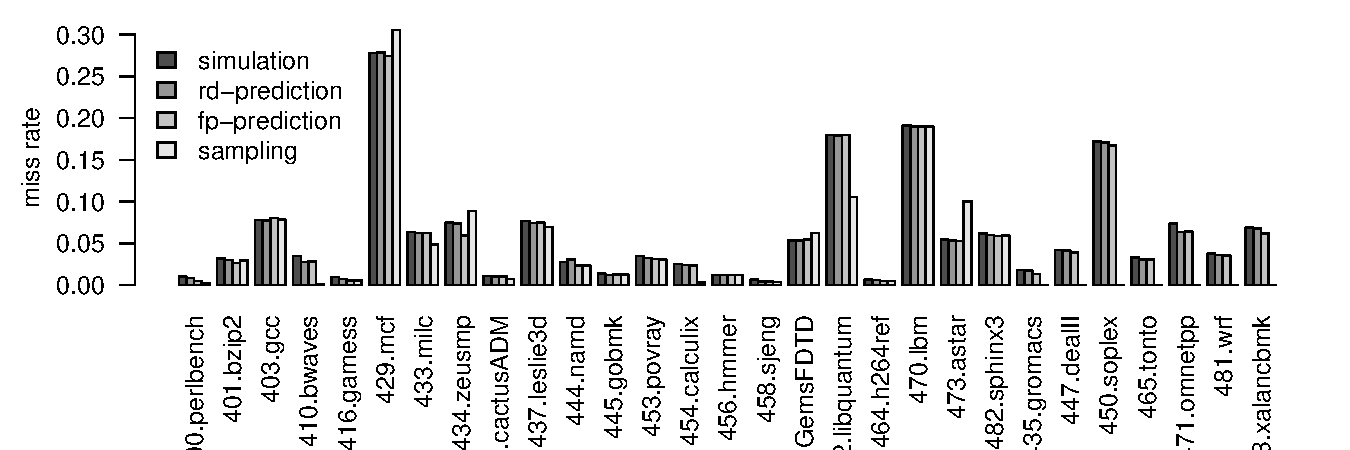
\includegraphics[width=0.85\textwidth]{figures/model/spec_l1}
  }
  \subfigure[8-way, 256KB cache]{
    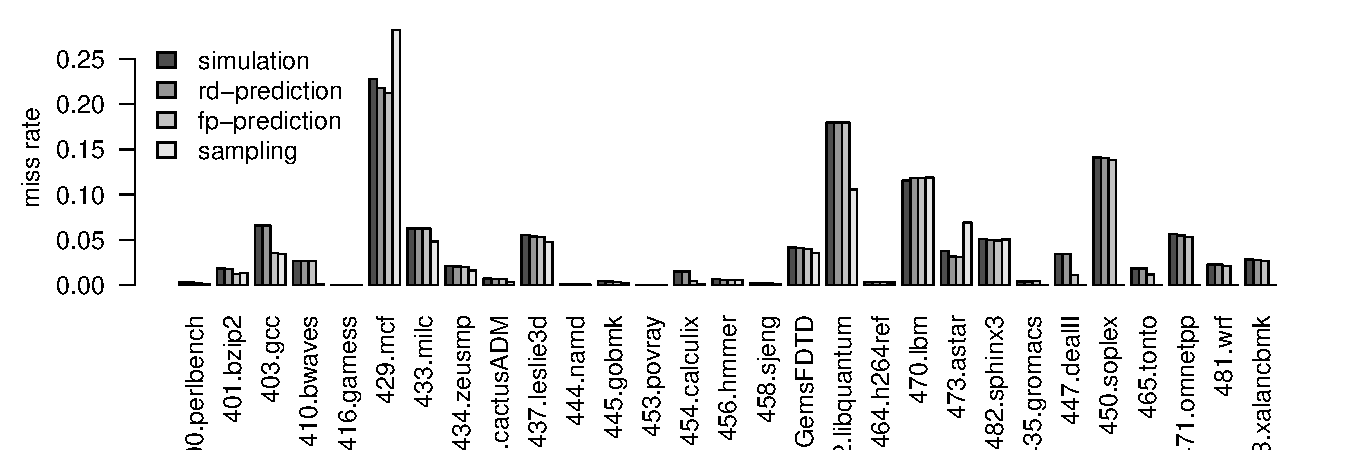
\includegraphics[width=0.85\textwidth]{figures/model/spec_l2}
  }
  \subfigure[16-way, 8MB cache]{
    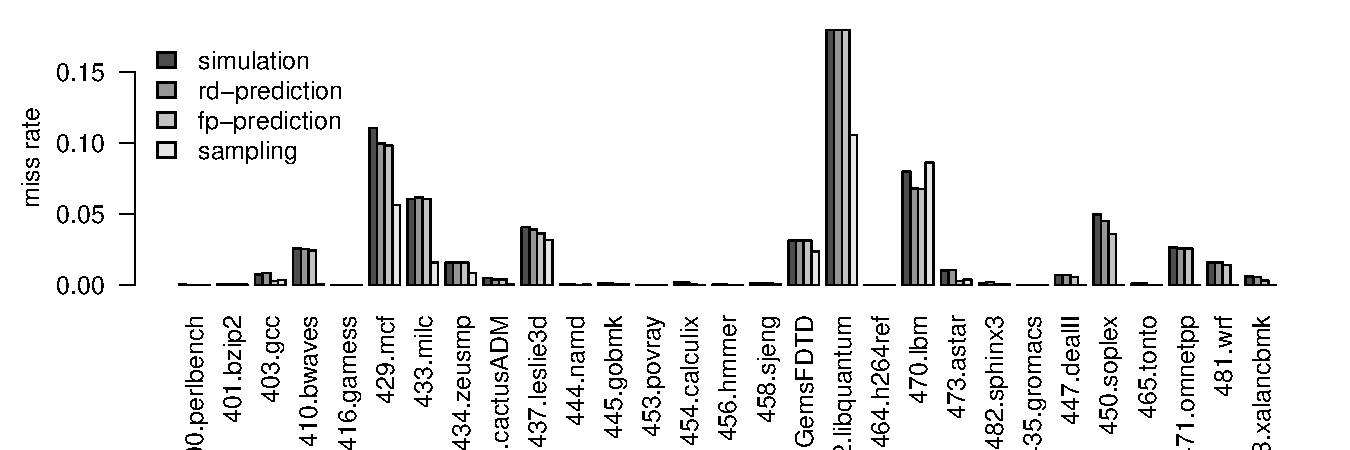
\includegraphics[width=0.85\textwidth]{figures/model/spec_l3}
  }
  \caption{Accuracy of the miss-ratio prediction by reuse distance,
    footprint (HOTL conversion in Section~\ref{subsec:mr}), and footprint sampling
    (Section~\ref{sec:sampling-phase}) for 29 SPEC 2006 benchmarks, each on
    3 (of the 3073) cache configurations, compared with cache
    simulation.  (a) 8-way, 32KB cache.  (b) 8-way, 256KB cache.  (c)
    16-way, 8MB cache.  The sampling results are for 22 out of 29
    programs (not the last 7).  The average time cost of sampling is
    0.5\% (Table~\ref{tbl:speed}).}
  \label{fig:spec_pred}
\end{figure} 

We first use cache simulation to evaluate the accuracy of Filmer-based
miss ratio prediction.  Instead of evaluating each of the 29 programs
on 3073 cache sizes, we show results for 3 configurations: 32KB, 8-way
associative L1D; 256KB, 8-way associative L2; and 8MB, 16-way
associative L3. They are the cache configurations on our test
machine. We will compare our prediction to the performance counter
result later. The cache-block size is 64 bytes in all cases.  The
accuracy for the other 3070 cache sizes looks similar.

Figure~\ref{fig:spec_pred} plots the measured and predicted miss ratios.
The \emph{rd-prediction}, which uses the measured reuse distance, is the
most accurate.  The other two, \emph{fp-prediction} and \emph{sampling}
measure the footprint and then use the HOTL conversion in
Section~\ref{subsec:mr}.  The HOTL conversion \emph{fp-prediction}
closely matches the reuse-distance analysis \emph{rd-prediction} in
almost all cases, showing that the footprint-converted reuse distance
is almost identical to the measured reuse distance---hence the
validity of the reuse-window hypothesis.  

\paragraph{The phase effect}
The reuse distances of a program, when added together regardless of
phases, predict the (capacity) miss ratio accurately, because an
access is a cache capacity miss if and only if its reuse distance is
greater than the cache size.  On the other hand, the footprint should
be affected by phases.  As the footprint changes from phase to phase,
it is possible that taking the global average might lose critical
information.

A consistent result from the theory and the experiments is that the
two are largely equivalent, as far as computing the miss ratio is
concerned.  The theory gives the conversion procedure from the
footprint to the reuse distance.  The experiments show, by the
close match between \emph{rd-prediction} and \emph{fp-prediction} in
Figure~\ref{fig:spec_pred}, the conversion is accurate for most
programs.  This suggests that reuse windows are representative of all
windows, and this is why the prediction is accurate in spite of the
phase effect.

Another evidence, for which we do not include the results in the
paper, is that the two sampling designs in Section~\ref{sec:sampling-phase},
phase sensitive and insensitive, produce almost identical predictions.

\paragraph{Analysis speed}
Table~\ref{tbl:speed} compares the cost of four analysis methods: the
simulation
$sim$, the reuse distance $rd$~\cite{Zhong+:TOPLAS09}, the footprint
$fp$~\cite{Xiang+:PACT11}, and the footprint sampling $sp$.  For simulation we could use the
algorithm of Smith and Hill~\cite{HillS:TOC89} to simulate all three
configurations in one pass.  For speed comparison, we ran the simplest
simulator once for each configuration.  The simulation cost in
table~\ref{tbl:speed} is the average of the three runs.

The cost for reuse distance analysis ranges from 52 times to 426 times
with an average of 153 times.  The footprint analysis costs about 7
times less, with slowdowns between 6 and 66 times and on average 23
times.  Simulation for a single configuration has slowdowns from 14 to
80 times, with an average of 38 times.

Comparing the average, we see that measuring the footprint, the third
order Filmer metric that can compute the second order metric miss
ratio for all cache sizes, is 39\% faster than simulating for a single
cache size, before we use footprint sampling.

\begin{comment}
\begin{table}
\small
\centering
\begin{tabular}{|c|c|c|c|c|c|}
\hline
$bench name$ & $sim$ & $rd$ & $fp$ & $samp$ & $cov$ \\ \hline \hline
400.perlbench & 49 & 219 & 34 & 0.24\% & 3.1\% \\ \hline
401.bzip2 & 34 & 139 & 24 & 0.73\% & 1.5\% \\ \hline
403.gcc & 24 & 88 & 15 & 0.55\% & 0.1\% \\ \hline
410.bwaves & 57 & 196 & 35 & 2.14\% & 0.5\% \\ \hline
416.gamess & 62 & 286 & 40 & 0.29\% & 2.9\% \\ \hline
429.mcf & 10 & 56 & 6 & 0.14\% & 0.03\% \\ \hline
433.milc & 21 & 74 & 9 & 1.53\% & 0.04\% \\ \hline
434.zeusmp & 25 & 102 & 14 & 0.81\% & 0.06\% \\ \hline
435.gromacs & 40 & 142 & 19 & - & - \\ \hline
436.cactusADM & 40 & 167 & 21 & 0.00\% & 1.1\% \\ \hline
437.leslie3d & 42 & 131 & 23 & 0.00\% & 0.01\% \\ \hline
444.namd & 44 & 155 & 24 & 0.00\% & 2.2\% \\ \hline
445.gobmk & 35 & 130 & 23 & 0.22\% & 1.1\% \\ \hline
447.dealII & 54 & 209 & 34 & - & - \\ \hline
450.soplex & 13 & 52 & 7 & - & - \\ \hline
453.povray & 51 & 220 & 33 & 0.00\% & 1.8\% \\ \hline
454.calculix & 39 & 127 & 19 & 0.11\% & 1.8\% \\ \hline
456.hmmer & 80 & 426 & 59 & 0.00\% & 0.8\% \\ \hline
458.sjeng & 34 & 152 & 23 & 0.82\% & 0.4\% \\ \hline
459.GemsFDTD & 42 & 181 & 21 & 1.28\% & 0.01\% \\ \hline
462.libquantum & 17 & 48 & 9 & 0.00\% & 0.01\%\\ \hline
464.h264ref & 101 & 424 & 66 & 0.00\% & 1.2\% \\ \hline
465.tonto & 52 & 168 & 30 & - & - \\ \hline
470.lbm & 14 & 76 & 6 & 0.00\% & 0.01\% \\ \hline
471.omnetpp & 17 & 69 & 10 & - & - \\ \hline
473.astar & 15 & 73 & 11 & 0.80\% & 0.9\% \\ \hline
481.wrf & 33 & 113 & 19 & - & - \\ \hline
482.sphinx3 & 30 & 117 & 16 & 0.59\% & 1.2\%\\ \hline
483.xalancbmk & 31 & 99 & 21 & - & - \\ \hline
average & 38 & 153 & 23 & 0.47\% & 0.9\%\\ \hline
\end{tabular}
\caption{Time comparison between different profiling methods and
  cache simulation for SPEC 2006.
  The baseline is the execution time without any 
  instrumentation or analysis. The middle four columns show the
  slowdown compared to the baseline:
$sim$ for simulating one cache size, $rd$
 for reuse distance profiling, $fp$ for footprint profiling, and
  $samp$ for footprint sampling.  The last column $cov$ gives the sampling coverage.
}
\label{tbl:speed}
\end{table}
\end{comment}

\begin{table}
\small
\centering
\begin{tabular}{|c|c|c|c|c|c|c|c|c|c|c|c|c|}
\hline
$bench$ & $sim$ & $rd$ & $fp$ & $sp$ & $cov$ & $bench$ & $sim$ & $rd$ & $fp$ & $sp$ & $cov$ \\
$name$ & & & & (\%) & (\%) &$name$ & & & & (\%) & (\%) \\ \hline \hline
400.perl & 49 & 219 & 34 & 0.24 & 3.1 & 453.povr & 51 & 220 & 33 & 0.00 & 1.8 \\ \hline
401.bzip & 34 & 139 & 24 & 0.73 & 1.5 & 454.calc & 39 & 127 & 19 & 0.11 & 1.8 \\ \hline
403.gcc & 24 & 88 & 15 & 0.55 & 0.1 & 456.hmme & 80 & 426 & 59 & 0.00 & 0.8 \\ \hline
410.bwav & 57 & 196 & 35 & 2.14 & 0.5 & 458.sjen & 34 & 152 & 23 & 0.82 & 0.4 \\ \hline
416.game & 62 & 286 & 40 & 0.29 & 2.9 & 459.Gems & 42 & 181 & 21 & 1.28 & 0.01 \\ \hline
429.mcf & 10 & 56 & 6 & 0.14 & 0.03 & 462.libq & 17 & 48 & 9 & 0.00 & 0.01\\ \hline
433.milc & 21 & 74 & 9 & 1.53 & 0.04 & 464.h264 & 101 & 424 & 66 & 0.00 & 1.2 \\ \hline
434.zeus & 25 & 102 & 14 & 0.81 & 0.06 & 465.tont & 52 & 168 & 30 & - & - \\ \hline
435.grom & 40 & 142 & 19 & - & - & 470.lbm & 14 & 76 & 6 & 0.00 & 0.01 \\ \hline
436.cact & 40 & 167 & 21 & 0.00 & 1.1 & 471.omne & 17 & 69 & 10 & - & - \\ \hline
437.lesl & 42 & 131 & 23 & 0.00 & 0.01 & 473.asta & 15 & 73 & 11 & 0.80 & 0.9 \\ \hline
444.namd & 44 & 155 & 24 & 0.00 & 2.2 & 481.wrf & 33 & 113 & 19 & - & - \\ \hline
445.gobm & 35 & 130 & 23 & 0.22 & 1.1 & 482.sphi & 30 & 117 & 16 & 0.59 & 1.2\\ \hline
447.deal & 54 & 209 & 34 & - & - & 483.xala & 31 & 99 & 21 & - & - \\ \hline
450.sopl & 13 & 52 & 7 & - & - & {\bf average} & {\bf 38} & {\bf 153} & {\bf 23} & {\bf 0.47} & {\bf 0.9}\\ \hline
\end{tabular}
\caption{Time comparison between different profiling methods and
  cache simulation for SPEC 2006.
  The baseline is the execution time without any 
  instrumentation or analysis. The middle four columns show the
  slowdown compared to the baseline:
$sim$ for simulating one cache size, $rd$
 for reuse distance profiling, $fp$ for footprint profiling, and
  $samp$ for footprint sampling.  The last column $cov$ gives the sampling coverage.
}
\label{tbl:speed}
\end{table}


\paragraph{Locality sampling}
\label{sec:samp-result}

For this experiment, we choose somewhat arbitrarily the frequency of
one sample every 10 seconds.  The sample length is the volume fill
time for the cache size.  Sampling analysis is not always accurate.
Visible errors are seen in \emph{mcf}, \emph{libquantum} and
\emph{astar} in Figure~\ref{fig:spec_pred}.  The reason, as shown by
the last column of Table~\ref{tbl:speed}, is that it covers less than
1\% of the execution.  The coverage is computed by the ratio of the
number of sampled instructions to the total number of instructions
(counted by our full trace profiling).  The coverage is as low as
0.006\% in \emph{lbm}.  The low coverage does not mean low
accuracy. The prediction of \emph{lbm} is 99\% accurate for the 32KB
cache, 97\% for the 256KB cache, and 92\% for the 8MB cache.

% Neither does the low coverage mean low cost.  

In Table~\ref{tbl:speed}, we show the slowdown in the end-to-end run
time by the column marked $samp$.  It ranges from 0\% to 2.14\%. Three
programs have a visible cost of over 1\%.  They are \emph{bwaves}
2.1\%, \emph{GemsFDTD} 1.3\% and \emph{milc} 1.5\%.  The reason for
the relatively high cost may be the non-trivial interference between
the sampling task and the parent task.  Across all programs, the
average visible overhead is below a half percent. If we measure the
total CPU time, sampling takes between 0\% and 80\% of the original
run time.  The average cost is 19\%, of which over 18\% is hidden by
shadow profiling. 

\paragraph{Parallel programs}
Figure~\ref{fig:parsec_pred} shows that for 3 of the 3073 cache
configurations and across the 3 input sizes, the predicted miss ratio
matches closely with the simulated miss ratio, similar to the results
we saw in the sequential programs.  The accuracy shows that the
reuse-window hypothesis holds for these threaded applications.

The last column of table~\ref{tbl:parsec_basic} shows the slowdowns of
footprint profiling, which ranges from 14 times to 159 times with an average
of 113 times.  We did not profile reuse distance for PARSEC because it took
too long.  We note that the footprint analysis shows 5 times as much
overhead in 4-threaded tests as in sequential programs (159 times in
PARSEC vs. 23 times in SPEC
2006).  The reason is that our data analysis is still serial, so the
overhead is proportional to the total amount of work.  We plan to
parallelize the footprint analysis in the future, building on recent
work in parallelizing the reuse-distance analysis~\cite{Cui+:IPDPS12,
Gupta+:IPDPS12,Niu+:IPDPS12}.

\begin{figure}[h!]
  \centering
  \subfigure[8-way, 32KB cache]{
    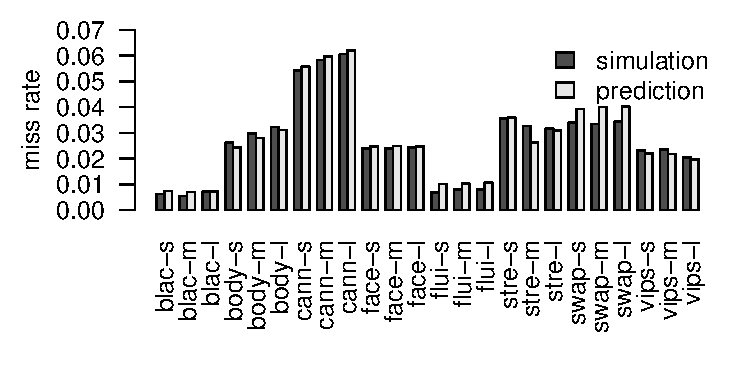
\includegraphics[width=0.7\textwidth]{figures/model/parsec_l1}
  }
  \subfigure[8-way, 256KB cache]{
    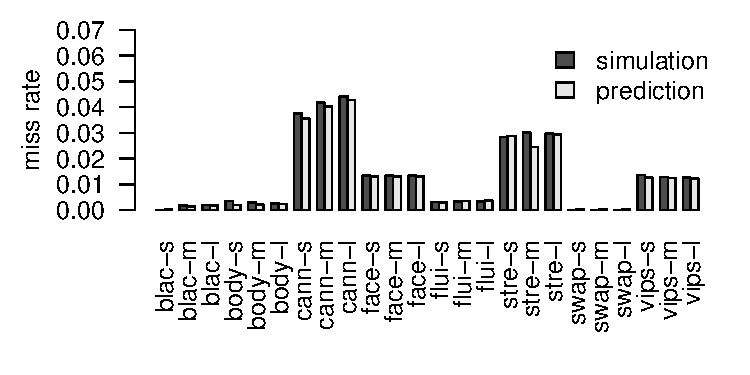
\includegraphics[width=0.7\textwidth]{figures/model/parsec_l2}
  }
  \subfigure[16-way, 8MB cache]{
    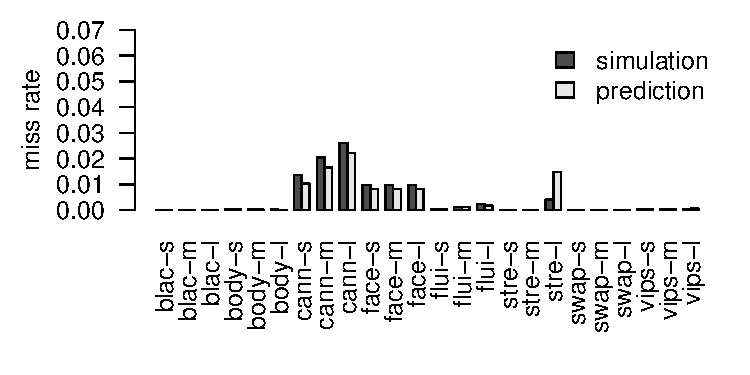
\includegraphics[width=0.7\textwidth]{figures/model/parsec_l3}
  }
  \caption{Accuracy of the miss-ratio prediction for 3 (of the 3073) cache
    configurations and 3 input sizes, compared with cache simulation.  (a) 8-way, 32KB
    cache.  (b) 8-way, 256KB cache.  (c) 16-way, 8MB cache.}
  \label{fig:parsec_pred}
\end{figure} 

\begin{table}
\small
\centering
\begin{tabular}{|l|c|c|c|c|c|}
\hline
$bench name$ & $input size$ & $n$ $(10^9)$ & $m$ $(10^6 bytes)$ & $T(sec)$ & slowdown \\ \hline \hline 
blackscholes &S& 0.1 & 0.4 & 0.093 & 129 \\ \cline{2-6}
 &M& 0.4 & 1.2 & 0.384 & 91 \\ \cline{2-6}
 &L& 1.6 & 4.4 & 1.542 & 88 \\ \hline
bodytrack &S& 0.3 & 8.1 & 0.285 & 129 \\ \cline{2-6}
 &M& 1.1 & 11.1 & 0.948 & 155 \\ \cline{2-6}
 &L& 4.0 & 14.8 & 3.35 & 111 \\ \hline
canneal &S& 0.6 & 43.0 & 1.525 & 19 \\ \cline{2-6}
 &M& 1.3 & 84.3 & 3.859 & 15 \\ \cline{2-6}
 &L& 2.7 & 164.9 & 8.804 & 14 \\ \hline
facesim &S& 12.7 & 344.2 & 7.448 & 139 \\ \cline{2-6}
 &M& 12.7 & 344.2 & 7.306 & 131 \\ \cline{2-6}
 &L& 12.7 & 344.2 & 7.86 & 116 \\ \hline
fluid animate &S& 0.5 & 10.5 & 0.429 & 114 \\ \cline{2-6}
 &M& 1.3 & 20.6 & 0.983 & 145 \\ \cline{2-6}
 &L& 3.9 & 57.6 & 2.9 & 124 \\ \hline
stream cluster &S& 0.5 & 1.2 & 0.722 & 87 \\ \cline{2-6}
 &M& 2.6 & 2.9 & 1.641 & 138 \\ \cline{2-6}
 &L& 9.6 & 9.5 & 6.951 & 173 \\ \hline
swaptions &S& 3.6 & 0.9 & 2.349 & 134 \\ \cline{2-6}
 &M& 1.4 & 1.2 & 0.935 & 114 \\ \cline{2-6}
 &L& 5.7 & 1.9 & 3.766 & 132 \\ \hline
vips &S& 1.0 & 13.5 & 0.748 & 159 \\ \cline{2-6}
 &M& 3.1 & 26.9 & 2.228 & 140 \\ \cline{2-6}
 &L& 8.6 & 15.7 & 7.332 & 103 \\ \hline
\end{tabular}
\caption{The PARSEC parallel benchmarks. 
  For each benchmark, $n$ is the memory trace length of whole execution, $m$ is 
  the size of program data (in bytes) accessed during the execution, and $T$ is the
  execution time without any instrumentation or analysis.  The last
  column is the slowdown of
  the footprint analysis.}
\label{tbl:parsec_basic}
\end{table}


\subsection{Validation on a Real Machine}

In Figure~\ref{fig:counter}, we compare the simulation result with the
miss ratio measured by the hardware counters on our test machine. To
measure the actual misses, we use Intel's VTune tool to record three
hardware counter events named 

\medskip
\begin{tabular}{l}
\texttt{OFFCORE\_RESPONSE\_0.DATA\_IN.LOCAL\_DRAM} \\
\texttt{MEM\_INST\_RETIRED.LOADS} \\
\texttt{MEM\_INST\_RETIRED.STORES} \\
\end{tabular}
\smallskip

\noindent The measured miss ratio is the first count
divided by the sum of the last two counts.

The figure shows a significant difference in \emph{gcc}.  The reason
is that the simulation considers only data accesses but the hardware
counter counts instruction misses in the data cache, which we believe are significant in
\emph{gcc}.  

\begin{figure}[h!]
  \centering
  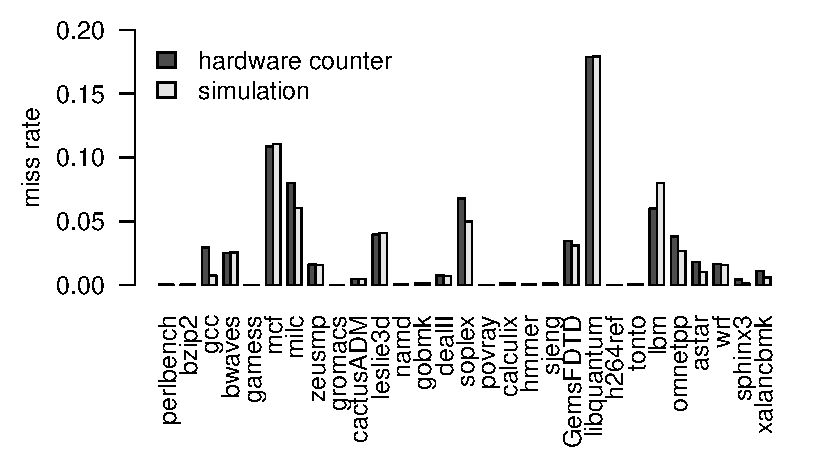
\includegraphics[width=0.8\textwidth]{figures/model/hwc_sim}
  \caption{Comparison between hardware counter measured L3 cache miss
    ratio and the simulation result.}
  \label{fig:counter}
\end{figure} 


\section{Discussion}
\label{sec:model_sum}
We proposed a higher order theory of locality to connect five
different locality metrics. The model endows each metric the strength
of all the other metrics. Give footprint's advantage of fast
measurement speed, we are able to get miss ratio of any cache size for
both sequential and parallel programs with very low overhead. This
technique is especially useful when we optimize system performance by
cache partitioning. The model also provides strong support for
evaluating cache sharing effect. We will bring cache sharing models
into the context in next Chapter and evaluate the model under cache
sharing environment. 
